\chapter{Problematyka zagadnienia w świetle literatury}
\label{ch:problematyka}

\section{Charakterystyka choroby Parkinsona}
\label{sec:charakterystykaPD}
Choroba Parkinsona (PD) jest zwyrodnieniowym schorzeniem mózgu związanym z objawami motorycznymi (spowolnienie ruchowe,
drżenie, sztywność, zaburzenia chodu i równowagi) oraz szeroką gamą powikłań niemotorycznych (zaburzenia poznawcze,
zaburzenia psychiczne, zaburzenia snu oraz ból i inne zaburzenia sensoryczne).
Zaburzenia motoryczne, takie jak dyskinezy (ruchy mimowolne) i dystonie (bolesne mimowolne skurcze mięśni) przyczyniają
się do ograniczenia mowy, mobilności i ograniczeń w wielu dziedzinach życia.
Postęp tych objawów powoduje wysoki stopień niepełnosprawności i konieczność opieki.
U wielu osób z PD w trakcie trwania choroby rozwija się również demencja.

Ryzyko zachorowania na PD rośnie wraz z wiekiem, chociaż choroba może dotyczyć także młodszych osób.
Bardziej narażeni są mężczyźni niż kobiety.
Przyczyna PD nie jest znana, ale uważa się, że powstaje w wyniku złożonej interakcji pomiędzy czynnikami genetycznymi i
narażeniem na czynniki środowiskowe, takie jak pestycydy, rozpuszczalniki i zanieczyszczenia powietrza przez całe życie.

Według raportu Światowej Organizacji Zdrowia\cite{WHO} w skali globalnej niepełnosprawność i zgony z powodu PD
rosną szybciej niż w przypadku jakichkolwiek innych zaburzeń neurologicznych.
Częstość występowania PD podwoiła się w ciągu ostatnich 25 lat.
Globalne szacunki w 2019 roku wykazały ponad 8,5 miliona osób z PD.
Obecne szacunki sugerują, że w 2019 roku PD spowodowała 5,8 miliona lat życia z niepełnosprawnością, co
stanowi wzrost o 81\% od 2000 roku, i spowodowała 329 000 zgonów, co stanowi wzrost o ponad 100\% od 2000 roku.


[DODAĆ WYKRES]


W Polsce z chorobą Parkinsona zmaga się około 100 tys. pacjentów, z czego około 20\% jest już w stadium zaawansowanym
według informacji przekazywanych przez Fundację Chorób Mózgu.
Ponadto co roku w naszym kraju wykrywanych jest ok. 8 tys. nowych zachorowań.
Nowe zachorowania nadal skorelowane są z wiekiem, średnia wieku chorych wynosi 60 lat, niestety wzrasta odsetek chorych wśród osób młodych (nawet w wieku 20 lat).




\subsection{Etapy Choroby}
\label{subsec:etapypd}


\subsection{Głos w chorobie Parkinsona}
\label{subsec:gospd}


\subsection{Problematyka choroby}
\label{subsec:problematykapd}


%---------------------------------------------------------------------------

\section{Przegląd dostępnych rozwiązań}
\label{sec:przeglad}

Diagnoza PD jest powszechnie oparta na obserwacjach lekarskich i ocenie objawów klinicznych, w tym charakterystyce różnorodnych objawów ruchowych.
Rosnąca liczba zachorowań i obniżenie wieku osób w grupie ryzyka, skutkuje wzrostem zainteresowania dotyczącym narzędzi, które ułatwiłyby
zarówno codzienne funkcjonowanie pacjentów jak i pracę lekarzy.
Tradycyjne metody diagnostyczne mogą być obarczone subiektywizmem ponieważ opierają się na ocenie ruchów, które są czasami subtelne dla
ludzkiego oka i dlatego trudne do sklasyfikowania, co może przyczynić się do błędnej diagnozy.
Ponadto wczesne objawy niemotoryczne PD mogą być łagodne oraz spowodowane wieloma innymi schorzeniami.
Dlatego też rozpoznanie tej choroby na wczesnym etapie stanowi wyzwanie.

Nie da się nie zauważyć, żę sztuczna inteligencja oraz nowoczesne technologie coraz częściej stają się integralną częścią systemu ochrony zdrowia.
Wspierają lekarzy podczas diagnozy oraz wyboru sposobu leczenia pacjenta,a także pozwalają na monitorowanie choroby.
Aby rozwiązać trudności i udoskonalić procedury diagnozowania oraz oceny PD, wdrożono metody uczenia maszynowego do klasyfikacji PD i osób zdrowych lub
pacjentów z podobnymi objawami klinicznymi (np. zaburzeniami ruchu lub innymi zespołami parkinsonowskimi).


W przeglądzie publikacji na temat wykorzystania uczenia maszynowego do diagnostyki PD do 2020 roku wyróżniono 209 artykułów\cite{ML_for_PD_review}.


%\begin{figure}[htbp]
%	\centering
%	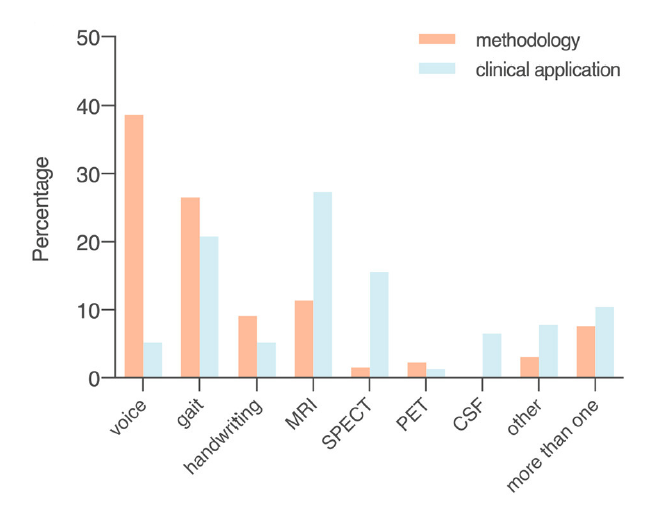
\includegraphics[width=0.7\textwidth]{./img/plot_PD_detection_methods}
%	\caption{Wykres przedstawiający rozkład rodzaju danych na których bazowały systemy ML do diagnostyki PD\cite{ML_for_PD_review} (stan na dzień 14 luty 2020)}
%    \label{fig:wykres_1}
%\end{figure}


\subsection{Rozwiązania teoretyczne}
\label{subsec:rozwiazania-teoretyczne}

\subsection{Aplikacje rzeczywiste}
\label{subsec:aplikacje}


\subsection{Wady istniejących rozwiązań}
\label{subsec:wady_rozwiazan}

Ostatnie badania wykazały, że możemy wytrenować dokładne modele do wykrywania oznak PD z nagrań audio.
Jednakże, istnieją rozbieżności pomiędzy badaniami i mogą być spowodowane, częściowo, przez różnice w
wykorzystywanych korpusach lub metodologii.
Dlatego w\cite{SustainedVowelsProblems} przeprowadzono analizę, która wykazała, że nieuwzględnione zmienne w metodologii,
projekcie eksperymentalnym i przygotowaniu danych doprowadziły do zbyt optymistycznych wyników w badaniach nad
automatyczną detekcją PD z wykorzystaniem podtrzymywanych samogłosek.
Przeprowadzono eksperymenty, które pozwoliły na sformułowanie kilku zasad zabezpieczających przed zbyt
optymistycznymi i mylącymi wynikami.
Zidentyfikowano następujące czynniki, jako wpływające na wyniki klasyfikacji:


\begin{enumerate}[label={\alph*)}]
	\item Wpływ tożsamości mówcy na dokładność klasyfikacji
	\item[] Im większa różnica między liczbą plików a wymiarem wektora cech, tym większe szanse na znalezienie cechy, która losowo koreluje z etykietami klas.
  	\item Wpływ różnicy wieku między klasami na dokładność klasyfikacji
	\item[] Różnica w średnim wieku mówców z oraz bez choroby Parkinsona może prowadzić do zbyt optymistycznych wyników, ponieważ
związany z wiekiem wpływ na głos mówców może wpływać na klasyfikator.

  	\item Wpływ losowości cech na dokładność klasyfikacji
  	\item Łagodzenie losowego nadmiernego dopasowania przy użyciu danych programistycznych
	\item Wpływ rozpoczęcia i przesunięcia samogłosek na wyniki klasyfikacji
 	\item Eksperymenty międzykorporowe
	\item Analiza cech
\end{enumerate}



%\begin{figure}[htbp]
%	\centering
%	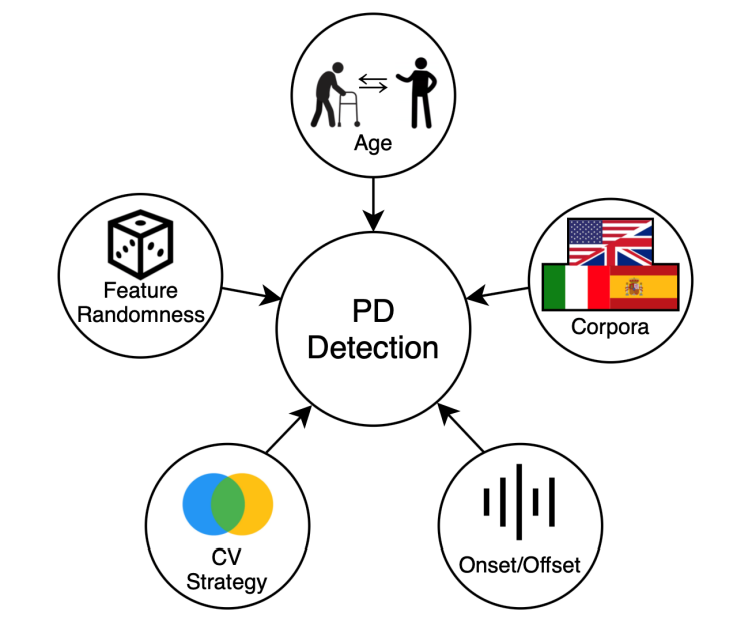
\includegraphics[width=0.7\textwidth]{./img/influence_of_factos_on_PD_detection}
%	\caption{Czynniki wpływające na dokładność detekcji Parkinsona na podstawie głosu]}
%    \label{fig:wykres_2}
%\end{figure}


Nie są to jednak wszystkie czynniki, które zaburzają obiektywność wyników. Konieczna jest dyskusja na temat nowych
kompleksowych linii bazowych dla prowadzenia eksperymentów w automatycznym wykrywaniu PD na podstawie fonacji,
a także innych ogólnych zastosowań przetwarzania mowy.


\subsection{Wnioski}
\label{subsec:wnioski}

Prace nad automatyczną detekcją Parkinsona na podstawie głosu trwają już od dłuższego czasu.
Jednak wciąż brakuje systemu, który mógłby zostać uznany jako wystarczajaco niezawodne narzędzie diagnostyczne.
Wśród problemów, które ograniczają rzeczywiste wykorzystanie takich systemów wyróżnia się:

%---------------------------------------------------------------------------
